%% abtex2-modelo-livro.tex, v<VERSION> 
%% Copyright 2012-<COPYRIGHT_YEAR> by abnTeX2 group at http://www.abntex.net.br/
%%
%% This work may be distributed and/or modified under the
%% conditions of the LaTeX Project Public License, either version 1.3
%% of this license or (at your option) any later version.
%% The latest version of this license is in
%%   http://www.latex-project.org/lppl.txt
%% and version 1.3 or later is part of all distributions of LaTeX
%% version 2005/12/01 or later.
%%
%% This work has the LPPL maintenance status `maintained'.
%%
%% Further information is available on 
%% http://www.abntex.net.br/
%% 


\documentclass[
% -- opções da classe memoir --
12pt,				% tamanho da fonte
openright,			% capítulos começam em pág ímpar (insere página vazia caso preciso)
oneside,			% para impressão em recto e verso. Oposto a oneside
a4paper,			% tamanho do papel. 
% -- opções da classe abntex2 --
%chapter=TITLE,		% títulos de capítulos convertidos em letras maiúsculas
%section=TITLE,		% títulos de seções convertidos em letras maiúsculas
%subsection=TITLE,	% títulos de subseções convertidos em letras maiúsculas
%subsubsection=TITLE,% títulos de subsubseções convertidos em letras maiúsculas
% -- opções do pacote babel --
%english,			% idioma adicional para hifenização
%french,				% idioma adicional para hifenização
brazil,				% o último idioma é o principal do documento
sumario=tradicional
]{abntex2}

%licença de uso
\usepackage{ccicons}

% compilação de fontes
\usepackage{mathtools}
\usepackage{amsfonts}
\usepackage{mathrsfs} % para mathscr

\usepackage{ifxetex}
\ifxetex
% % se for utilizar as fontes do sistema: **escolha sua fonte**
% comandos de fontes
\usepackage{mathspec}
\setmathsfont(Digits,Latin,Greek){Minion Pro}
\setmathrm{Minion Pro}
%\setmainfont[Numbers=OldStyle]{Minion Pro} %fonte principal (serifada)
\setmainfont[Numbers=OldStyle]{Clear Sans} %fonte principal (serifada)
%\setsansfont[Scale=0.9]{Myriad Pro} %fonte sem serifas
\setsansfont[Scale=0.9]{Clear Sans Thin} %fonte sem serifas
\setmonofont[Scale=MatchLowercase]{Consolas} % fonte monoespaçada

\usepackage{polyglossia} %always load polyblossia after fonts for digits in math mode
\setmainlanguage{brazil}
\setotherlanguages{french,english,spanish,german,italian}  

\else
% % se for utilizar pdflatex
\usepackage[utf8]{inputenc}
\usepackage{newtxmath} 
\usepackage{Alegreya}
\usepackage{AlegreyaSans}
\usepackage[lf]{FiraMono}
\usepackage[italic]{mathastext}
\fi

%% Observação: o pacote polyglossia pode apresentar erro ao ser utilizado com ifxetex + babel. 
%% Se isso acontecer, atualize o pacote para a versão mais recente ou utilize somente uma das sequências (pdflatex ou xelatex), comentando ou apagando a outra.

\usepackage{microtype} 				% para melhorias de justificação
\usepackage[dvipsnames]{xcolor} 		% para cores
\usepackage{graphicx} 			% para imagens
\usepackage{booktabs,tabularx,rotating}	% para tabelas
\usepackage{mdframed} 				% para caixas de texto como na CIP do verso do título
\usepackage{multicol}				% tabelas com colunas mescladas
\usepackage{lettrine}				% letras capitulares
\usepackage{xspace} 				% para nao precisar de espaços com {} depois de comandos
% como \LaTeX e abreviações criadas pelo usuário
\usepackage{leading}				% espaçamento entrelinhas (leading)
\leading{13pt}

% ---
% Pacotes de citações
% ---
\usepackage[brazilian,hyperpageref]{backref}	 % Paginas com as citações na bibl
\def\chapterautorefname{capítulo}
\def\sectionautorefname{seção}
\def\subsectionautorefname{subseção}
\def\subsubsectionautorefname{subsubseção}
\def\figureautorefname{figura}
\def\tableautorefname{tabela}
\def\equationautorefname{equação}

\usepackage[alf]{abntex2cite}	% Citações padrão ABNT

% ---
% Configurações do pacote backref
% Usado sem a opção hyperpageref de backref
\renewcommand{\backrefpagesname}{Citado na(s) página(s):~}
% Texto padrão antes do número das páginas
\renewcommand{\backref}{}
% Define os textos da citação
\renewcommand*{\backrefalt}[4]{
	\ifcase #1 %
	Nenhuma citação no texto.%
	\or
	Citado na página #2.%
	\else
	Citado #1 vezes nas páginas #2.%
	\fi}%
% ---

% ---
% Informações do documento
% ---
\titulo{Sistema +2d6@IFSul: Livro de Regras}
\autor{José de Figueiredo}
\data{2024, v<2.0>}
\preambulo{Breve sinopse do livro}
\local{Passo Fundo}
\instituicao{Sem editora ainda}

% alterando o aspecto da cor azul
\definecolor{blue}{RGB}{41,5,195}

% informações do PDF
\makeatletter
\hypersetup{
	%pagebackref=true,
	pdftitle={\@title}, 
	pdfauthor={\@author},
	pdfsubject={\imprimirpreambulo},
	pdfcreator={LaTeX with abnTeX2},
	pdfkeywords={abnt}{latex}{abntex}{abntex2}{livro}, 
	colorlinks=true,       		% false: boxed links; true: colored links
	linkcolor=blue,          	% color of internal links
	citecolor=blue,        		% color of links to bibliography
	filecolor=magenta,      		% color of file links
	urlcolor=blue,
	bookmarksdepth=4
}
\makeatother
% ---


% ---
% Estilo de capítulos
%
%\chapterstyle{pedersen} 
%\chapterstyle{lyhne} 
\chapterstyle{madsen} 
%\chapterstyle{veelo} 
%
% Veja outros estilos em:
% https://www.ctan.org/tex-archive/info/MemoirChapStyles
% ---

% para cabeçalhos sem estar em maiúsculas
%\nouppercaseheads 

% -----
% Declarações de cabecalhos 
% -----
% Cabecalho padrao
\makepagestyle{abntbookheadings}
\makeevenhead{abntbookheadings}{\ABNTEXfontereduzida\thepage}{}{\ABNTEXfontereduzida\textit\leftmark}
\makeoddhead{abntbookheadings}{\ABNTEXfontereduzida\textit\rightmark}{}{\ABNTEXfontereduzida\thepage}
\makeheadrule{abntbookheadings}{\textwidth}{\normalrulethickness}

% Cabecalho do inicio do capitulo
\makepagestyle{abntbookchapfirst}
\makeoddhead{abntbookchapfirst}{}{}{}

% Configura layout para elementos textuais
\renewcommand{\textual}{%
	\pagestyle{abntbookheadings}%
	\aliaspagestyle{chapter}{abntbookchapfirst}% customizing chapter pagestyle
	\nouppercaseheads%
	\bookmarksetup{startatroot}% 
}
% ---

% Margens do documento 
%% (margens do abntex2 não combinam nem com A5 nem com estilos de capítulo da
% classe memoir.)
\setlrmarginsandblock{2.5cm}{3.5cm}{*}
\setulmarginsandblock{2.5cm}{3.5cm}{*}
\checkandfixthelayout
% ---

\setlength{\parskip}{0.2cm} % tente também \onelineskip
\OnehalfSpacing

% ---
% Início do documento
% ---
\begin{document}
	\frenchspacing
	
	\frontmatter
	
	% ---
	% Capa principal
	% ---
	\begin{titlingpage}
		\phantom{xxx}
		\vspace{0.5cm}
		\huge
		\raggedright
		\imprimirautor\\
		\vspace{2.5cm}
		\huge 
		{\raggedleft
			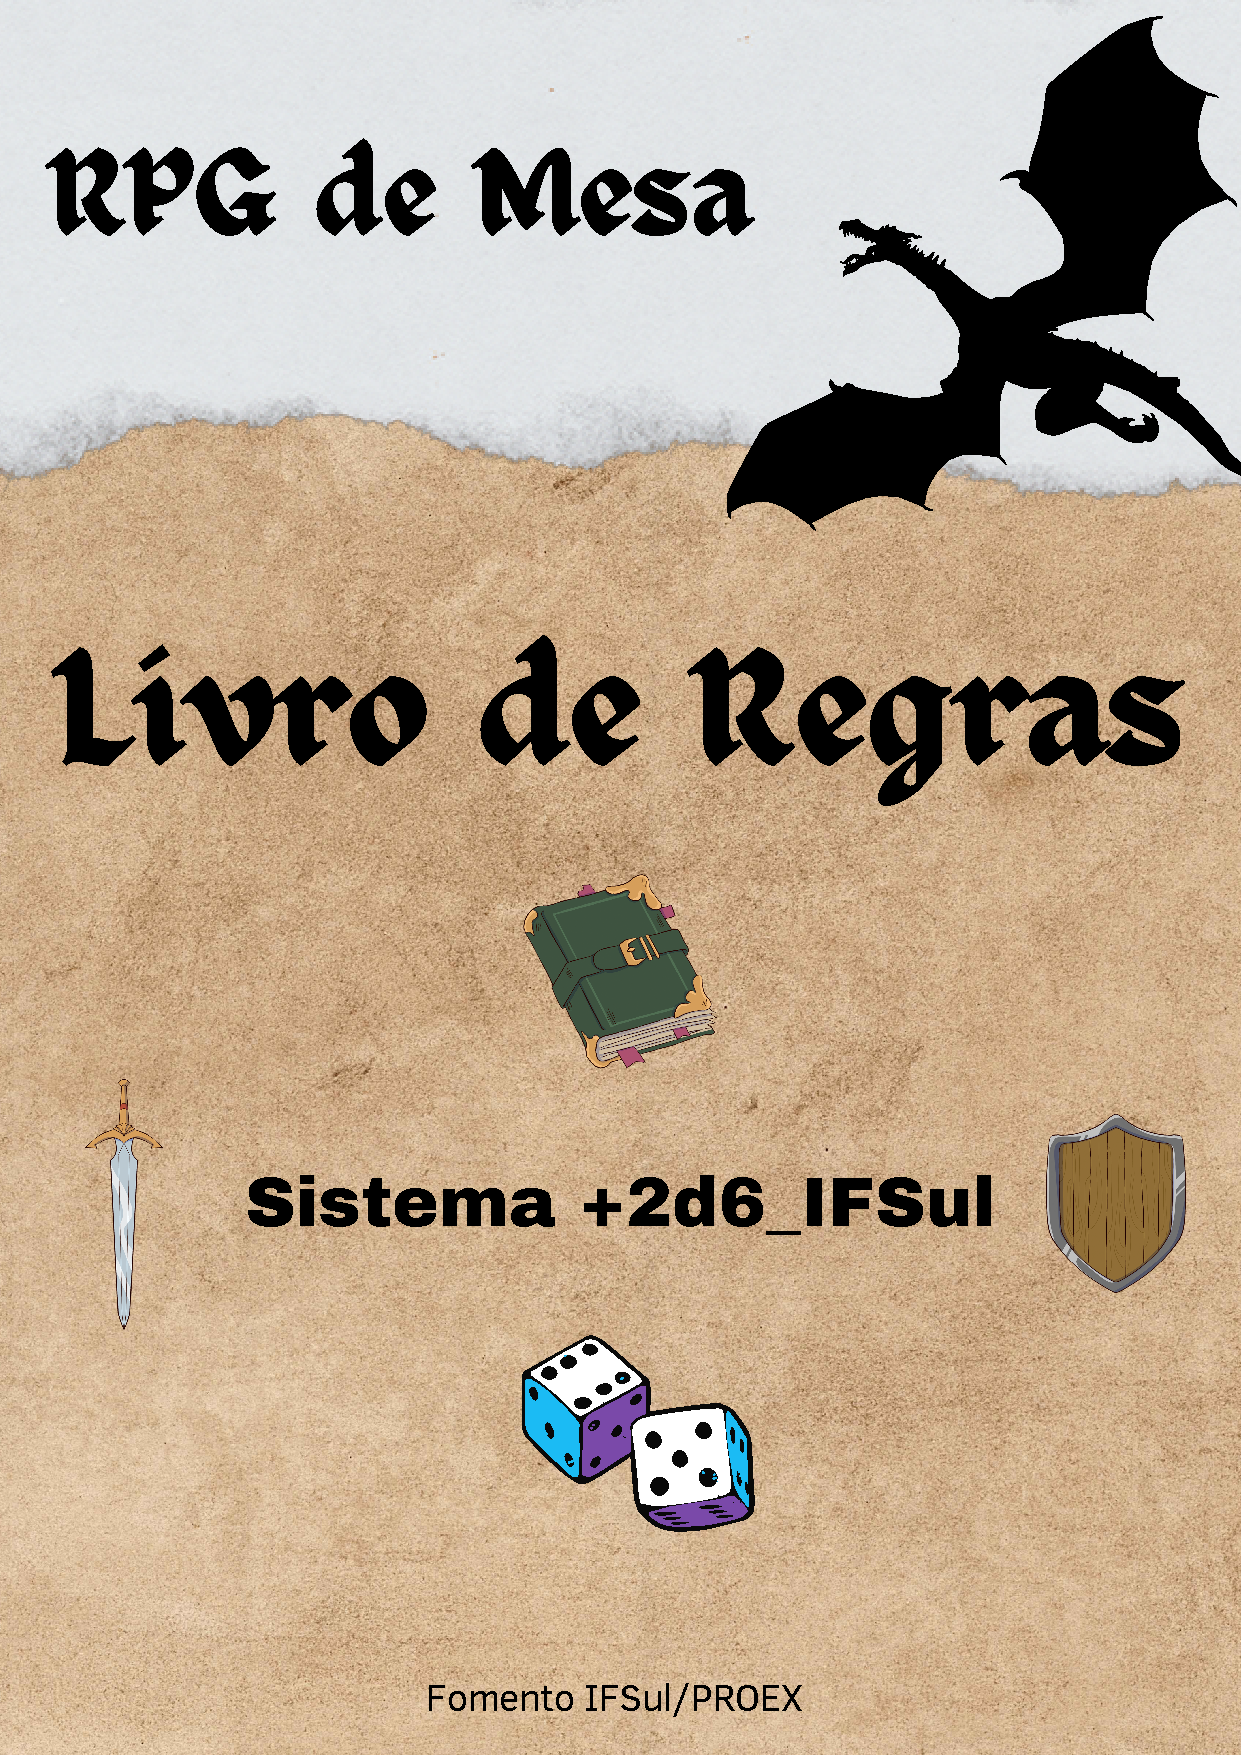
\includegraphics[scale=0.5]{img/capa.pdf}\\[1cm]
			\textit{\textcolor{blue}{\imprimirtitulo}}\\[1cm]
		}
		\centering 
		% %este é um símbolo que só aparecerá com a fonte Minion.
		\vfill
		\Large
		% %este é um símbolo que só aparecerá com a fonte Minion.
		\imprimirinstituicao
	\end{titlingpage}
	% ---
	
	% ---
	% Contra-capa
	% ---
	\begin{titlingpage}
		
		\phantom{xxx}
		\vspace{0.5cm}
		\huge
		\raggedright
		\imprimirautor\\
		\vspace{2.5cm}
		\huge 
		{\raggedleft
			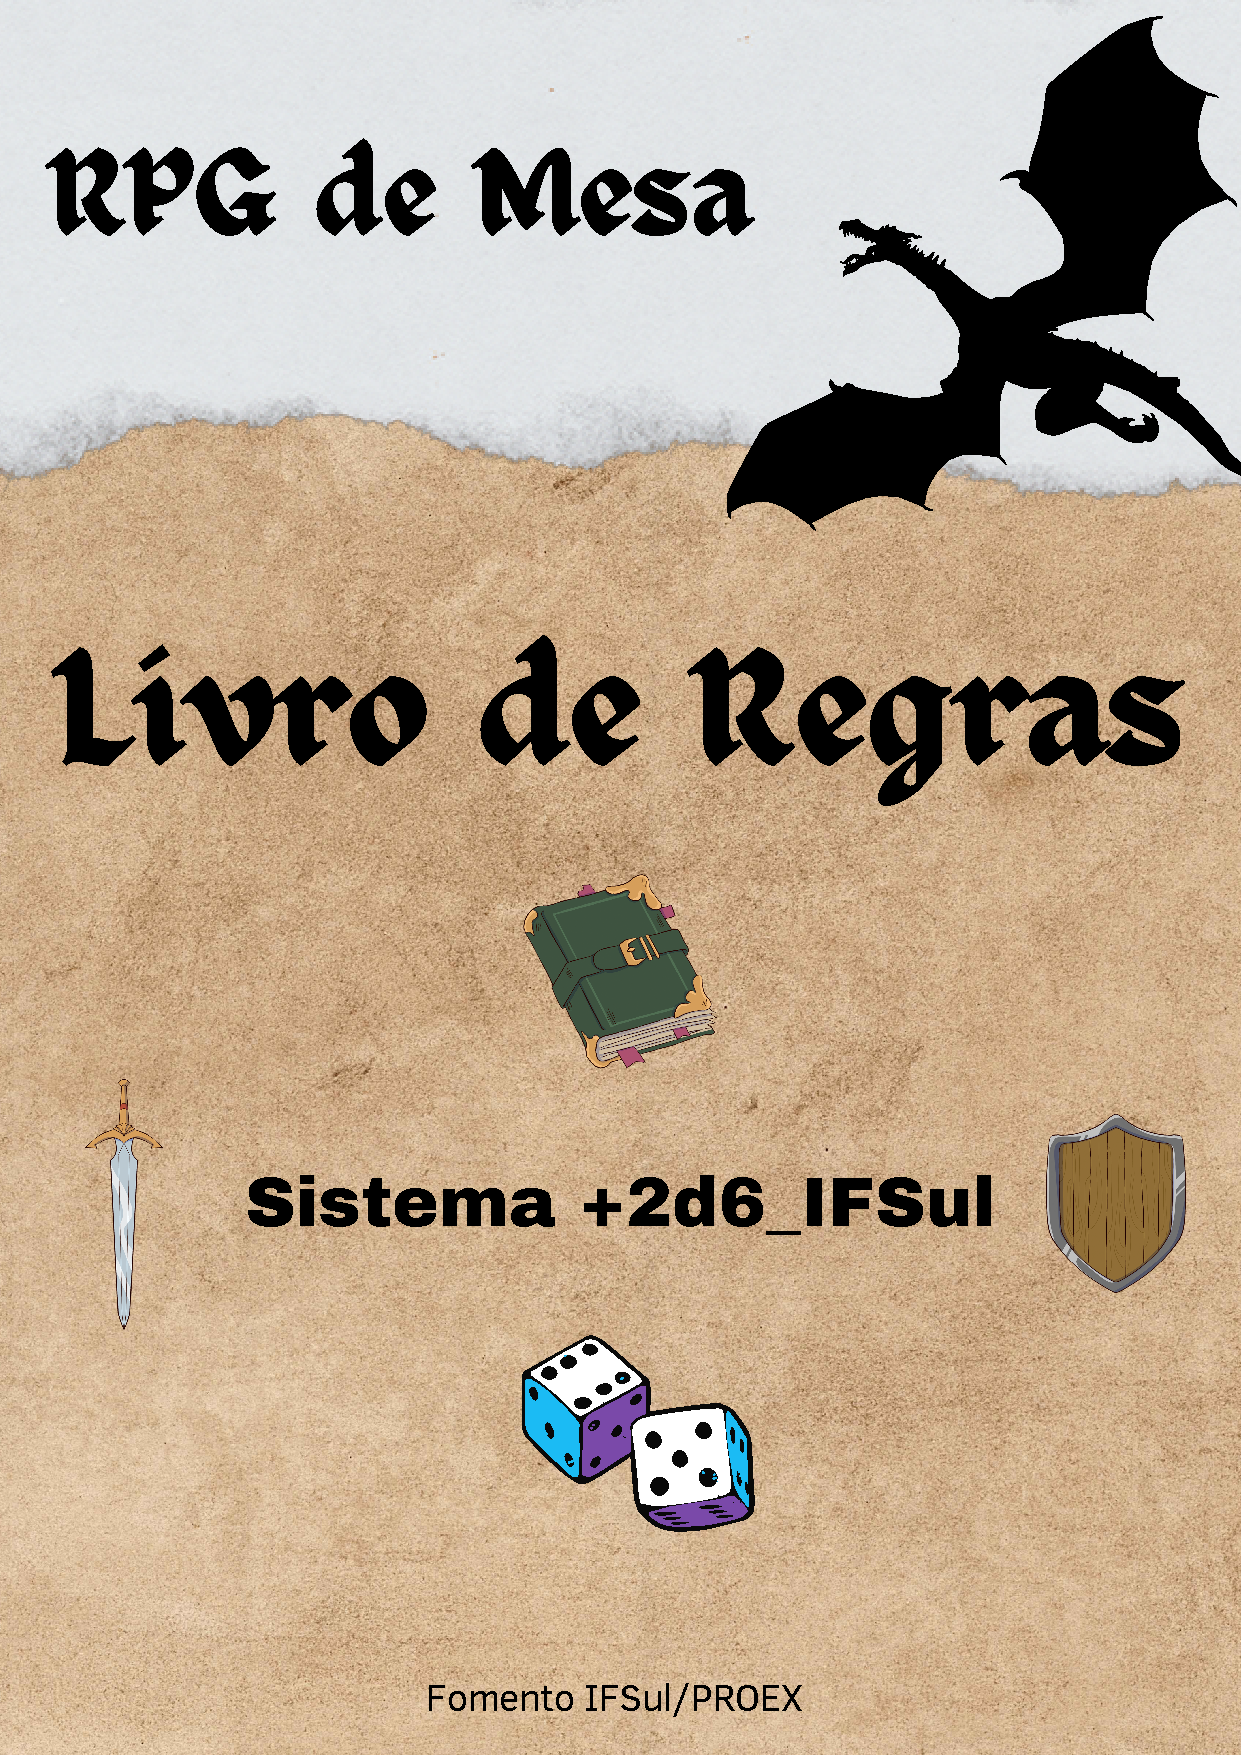
\includegraphics[scale=0.7]{img/capa.pdf}\\[1cm]
			\textit{\textcolor{blue}{\imprimirtitulo}}\\[1cm]
		}
		\centering 
		% %este é um símbolo que só aparecerá com a fonte Minion.
		\vfill
		\Large
		% %este é um símbolo que só aparecerá com a fonte Minion.
		\imprimirinstituicao
		% ---
		
		% ---
		% Verso da contra-capa
		% ---
		\clearpage
		\ABNTEXfontereduzida
		%\raggedright
		© 2017 \imprimirautor \space \& \imprimirinstituicao
		%este é só um exemplo de copyright.
		
		Qualquer parte desta publicação pode ser reproduzida, desde que citada a fonte.
		
		\vspace*{\fill}
		
		\begin{center}
			Dados Internacionais de Catalogação na Publicação (\textsc{cip})
			Câmara Brasileira do Livro, \textsc{sp}, Brasil
		\end{center}
		
		\begin{mdframed}
			\noindent Tal, Fulano de.
			
			\imprimirtitulo. / \imprimirautor. -- \imprimirlocal: \imprimirinstituicao
			Ltda., 2015.
			
			\medskip
			
			Bibliografia.
			
			ISBN XXXX-XXXX-XX.
			
			\medskip
			
			1. Programas de computador. 2. Tipografia. 3. Latex. 4. Normas ABNT.
			
		\end{mdframed}
		
	\end{titlingpage}
	% ---
	
	% ---
	% inserir lista de ilustrações
	% ---
	%\pdfbookmark[0]{\listfigurename}{lof}
	%\listoffigures*
	%\cleardoublepage
	
	% ---
	% inserir lista de tabelas
	% ---
	%\pdfbookmark[0]{\listtablename}{lot}
	%\listoftables*
	%\cleardoublepage
	% ---
	
	% ---
	% inserir o sumario
	% ---
	\pdfbookmark[0]{\contentsname}{toc}
	\tableofcontents*
	\cleardoublepage
	% ---
	
	% ------------------------------------------------------------
	% Início da parte textual
	% ------------------------------------------------------------
	%\textual
	\mainmatter
	% ------------------------------------------------------------

	\chapter[Apresentação]{\label{ch:apres}Apresentação}
%\addcontentsline{toc}{chapter}{Apresentação}

Este livro de regras surgiu após a finalização do projeto de extensão “RPG na Biblioteca Pública: Potencializando Talentos”, executado no segundo semestre de 2023, com apoio financeiro do Instituto Federal Sul-rio-grandense, pelo edital geral de fomento Nº 02/2023- PROEX. 

Na ocasião, a equipe envolvida buscava um sistema de RPG (sob licença livre/aberta), que pudesse ser adaptado às necessidades do projeto. Vários sistemas foram testados e avaliados, sendo que o sistema selecionado foi o +2d6, criado pelo prof. Newton Rocha (Tio Nitro)\footnote{\url{https://newtonrocha.wordpress.com/}}. 

Ainda em 2023, fizemos contato com o prof. Newton, que prontamente autorizou a adaptação, originando assim o \emph{Sistema +2d6\_IFSul} (Versão 1.0). Em 2024 este livro de regras é organizado, contendo a essa primeira versão revisada e renomeada para \emph{Sistema +2d6@IM}. A principal adaptação é relacionada aos atributos do personagem, que passa utilizar conceitos das \emph{Inteligências Múltiplas}, de Howard Gardner\footnote{The Theory of Multiples Intelligences (1987).}.

\textcolor{red}{Segundo a Teoria das Inteligências Múltiplas (Gardner, H. 1987) uma pessoa possui várias inteligências, que podem ser vistos como potencias humanos. }

O esforço para concretização, divulgação e utilização deste material, é nutrido por evidências e também pela (forte) crença, de que o RPG de Mesa possui grande potencial para o estímulo da leitura, do trabalho colaborativo e desenvolvimento da imaginação e criatividade.

\section{\label{sec:cred}Licenciamento} 
Esta seção apresenta os créditos e a licença de uso deste trabalho.

\subsection*{Atribuição de créditos}
Este trabalho é uma adaptação do \emph{Sistema +2d6}, desenvolvido por \href{http://newtonrocha.wordpress.com/}{Newton "Tio Nitro" Rocha}, originalmente licenciado com Creative Commons 3.0 \ccby.

\subsection*{Licenças paro o Sistema +2d6@IM}
\href{https://github.com/josefigueiredo/Sistema2d6-ifsul}{Sistema +2d6@IM}\footnote{Para efeitos de licenciamento, o \emph{Livro de Regras} e o \emph{Sistema +2d6@IM} são considerados o mesmo objeto, denominado apenas \emph{Sistema +2d6@IM}.} © 2024 by \href{https://josefigueiredo.github.io/}{José Antônio de Figueiredo} is licensed under \href{https://creativecommons.org/licenses/by-sa/4.0/?ref=chooser-v1}{Creative Commons Attribution-ShareAlike 4.0 International} \ccbysa.

Nesta licença você \textbf{tem o direito de:}
\begin{itemize}
	\item Compartilhar — copiar e redistribuir o material em qualquer suporte ou formato para qualquer fim, mesmo que comercial.
	\item Adaptar — remixar, transformar, e criar a partir do material para qualquer fim, mesmo que comercial.
\end{itemize}

O licenciante não pode revogar estes direitos desde que você respeite os termos da licença.

\textbf{De acordo com os termos seguintes:}\\
\begin{itemize}
	\item \ccAttribution \textbf{ Atribuição} — Você deve dar o crédito apropriado , prover um link para a licença e indicar se mudanças foram feitas. Você deve fazê-lo em qualquer circunstância razoável, mas de nenhuma maneira que sugira que o licenciante apoia você ou o seu uso.
	\item \ccShare \textbf{ CompartilhaIgual} — Se você remixar, transformar, ou criar a partir do material, tem de distribuir as suas contribuições sob a mesma licença que o original.
	\item \textbf{Sem restrições adicionais} — Você não pode aplicar termos jurídicos ou medidas de caráter tecnológico que restrinjam legalmente outros de fazerem algo que a licença permita.	
\end{itemize}

\textbf{Avisos:}
\begin{itemize}
	\item Você não tem de cumprir com os termos da licença relativamente a elementos do material que estejam no domínio público ou cuja utilização seja permitida por uma exceção ou limitação que seja aplicável.
	\item Não são dadas quaisquer garantias. A licença pode não lhe dar todas as autorizações necessárias para o uso pretendido. Por exemplo, outros direitos, tais como direitos de imagem, de privacidade ou direitos morais , podem limitar o uso do material.
\end{itemize}

	\chapter{\label{ch:rpg}RPG de Mesa}

O RPG de Mesa\footnote{Em inglês Role Playing Game} é um jogo cooperativo e de interpretação de papéis, idealizado por Gary Gygax (1974). Em um RPG há uma história com vários personagens, mistérios e conflitos. Os jogadores participam da história, interagindo com os personagens e com o ambiente/cenário, fazendo a história evoluir.

Um dos jogadores (chamado Mestre) narra a história, controla (e interpreta) os personagens do Mestre (PdM) e descreve/narra os eventos que acontecem conforme os outros personagens agem. Os demais jogadores controlam (e interpretam) os personagens do jogador (PdJ), que interagem com a história narrada e com os eventos decorridos. 

Dentro do jogo os personagens podem fazer praticamente qualquer coisa, como conversar com outros personagens, manipular objetos, resolver ou criar conflitos, viajar para lugares distantes, inventar máquinas, experimentar poções, ou qualquer outra coisa que seja possível dentro do universo da história e seja compatível com as capacidades do personagem.

O RPG de Mesa é uma forma de entretenimento que vai além do simples jogo, sendo também uma poderosa ferramenta para o desenvolvimento da criatividade, pois envolve atividades como criação de personagens, de narrativas, de cenários fictícios, etc, estimulando a imaginação de maneira profunda e envolvente.

\section{\label{sec:necessario}O que é preciso para jogar RPG}
De forma geral é preciso:
\begin{itemize}
	\item \textbf{Grupo de Jogadores}: Reúna um grupo de amigos ou pessoas interessadas.
	\item \textbf{Um Mestre}: É o jogador responsável por narrar (e às vezes criar) a história, controlar os PdM's, definir a dificuldade dos desafios e manter o jogo em andamento. O Mestre também toma decisões sobre o jogo, narrando as consequências das ações dos jogadores.
	\item \textbf{Um Sistema de RPG}: Um conjunto de regras que define como criar personagens, resolver conflitos e executar a mecânica do jogo. Este Livro de Regras apresenta o \underline{Sistema +2d6@ifsul, que é simples, livre e gratuito}. 	
	No mercado, existem vários outros sistemas, como: \emph{Tormenta 20}\footnote{\url{https://jamboeditora.com.br/categoria/rpg/tormenta20-rpg/}}, \emph{Ordem Paranormal}\footnote{\url{https://jamboeditora.com.br/produto/ordem-paranormal-rpg/}} e \emph{Old Dragon} 2\footnote{\url{https://www.burobrasil.com/produtos/old-dragon/}}. 
	\item \textbf{Fichas de Personagem}: Cada jogador precisará de uma ficha na qual são registrados atributos, habilidades, história e outras informações sobre seu personagem. O livro de regras geralmente fornece modelos de fichas.
	\item \textbf{Dados de RPG}: Os dados são usados para alguns tipos de testes durante o jogo. O Sistema +2d6@ifsul requer apenas 2 dados de 6 faces, sendo uma alternativa de fácil acesso.
	\item \textbf{Imaginação e Criatividade}: RPGs são jogos baseados em interações criativas, imaginadas (e vivenciadas) no Teatro da Mente.
	\item \textbf{Tempo e Respeito}: Jogos de RPG exigem respeito mútuo e alguma dedicação de tempo.
\end{itemize}


	\chapter{\label{ch:pdj}Personagem do Jogador}

O RPG de Mesa terá dois tipos de personagens: 
\begin{itemize}
	\item Personagens do Mestre (PdM's ou NPC): Os PdM's são criados e controlados pelo narrador da mesa. A criação de PdM's é apresentada no Capítulo~\ref{ch:mestre} - \emph{Área do Mestre}.

	\item Personagem do Jogador (PdJ): O PdJ é criado e controlado por um dos jogadores da mesa. Cada jogador controla pelo menos um personagem.
\end{itemize}

\section{\label{sec:pdj}Criando um PdJ}

Para criar um PdJ no Sistema +2d6@ifsul, recomenda-se fazer primeiro uma descrição em texto de como é este personagem. Todas estas características serão transformadas em valores numéricos registrados na Ficha de Personagem. Logicamente, quanto maior o valor numérico nestes elementos, mais poderoso é o personagem naquele aspecto.

Os principais pontos da ficha são: 

\begin{itemize}
	\item ATRIBUTOS: Explicados na seção~\ref{subsecAtributos}, representam as capacidades físicas e mentais do personagem.
	\item PERÍCIAS: Explicadas na seção~\ref{subsecPericias}, são habilidades/ofícios aprendidas/conquistadas pelo personagem antes da aventura. Novas perícias também poderão ser aprendidas durante a aventura, principalmente quando estas forem longas no formato de campanhas.
	\item VANTAGENS e DESVANTAGENS: Explicadas na seção~\ref{subsecVantagens}, são características/poderes que afetam o personagem. Vantagens auxiliam/ajudam em determinadas situações, enquanto desvantagens prejudicam/atrapalham.
\end{itemize}

A Figura~\ref{fichaMaoLivre} mostra uma Ficha de Personagem feita a mão livre. O Apêndice~\ref{apendiceFichas} mostra dois outros modelos para Ficha de personagem. 

\begin{figure}[htb]
	\centering
	\includegraphics[scale=0.5]{img/fichaManual.png}
	\caption{Exemplo de ficha feita a mão livre.}
	\label{fichaMaoLivre}
\end{figure}

\subsection{\label{subsecAtributos}Atributos}

\subsection{\label{subsecPericias}Perícias}
\subsection{\label{subsecVantagens}Vantagens e Desvantagens}
	\chapter{\label{ch:pericias}Perícias}

Perícias representam as especialidades e poderes especiais dos personagens, sendo sempre determinadas pelo tipo de aventura. Estas habilidades podem ser específicas ou genéricas, sendo que neste caso é preciso concordância de todos os jogadores da mesa.

Ao narrar uma aventura, o Mestre precisa determinar quais perícias podem existir naquele universo ficcional ainda antes da criação dos personagens. Isso é necessário para evitar situações como o personagem está em uma aventura no Velho Oeste, mas "comprou" a perícia \emph{Hacker de computadores}. Em outras palavras, é preciso que as perícias dos jogadores façam sentido no universo em que a aventura acontece. 

Recomenda-se que o Mestre faça uma lista com 15 a 20 perícias compatíveis com o tipo de aventura que será narrado, para a criação dos personagens. Neste momento os jogadores poderão "comprar" as perícias escolhidas com os pontos de perícia. 

O Sistema +2d6@ifsul (bem como o Sistema +2d6 original) permitem a criação de perícias personalizadas, entretanto, este Livro de Regras não discute este mecanismo. Para saber mais sobre este assunto o leitor poderá acessar as regras originais do Sistema +2d6\footnote{\url{https://newtonrocha.wordpress.com/sistema-de-rpg-2d6/}}.  

\section{\label{sec:usoPericia} Comprando e Usando perícias}
Durante o jogo, a perícia é usada de forma complementar a algum atributo, ou seja, é importante "alinhar" perícias com os atributos registrados na ficha. Desta forma, a descrição do personagem fica coerente com a pontuação na ficha.

Se eu tenho um personagem que possui mais força se comparado aos outros atributos é lógico (mas não obrigatório) que eu procure comprar perícias relacionadas a força.

\begin{center}
	====================================================
\end{center}

Ao lado do nome de cada perícia está o Atributo Básico, ao qual ela deve ser somada em um teste de ação ou oposto (ver mais na seção Jogadas de testes). 

Para efeitos de jogo, as perícias são classificadas em valores numéricos, da seguinte forma: (1) Iniciante, (2) Profissional, (3) Experiente, (4) Perito, (5) Expert.

As perícias apresentadas nas seções a seguir são sugestões comuns. Os jogadores de uma mesa podem criar novas perícias desde que todos os jogadores estejam de comum acordo.

Por exemplo: Na listagem seção~\ref{sec:perFisicos} existe a \emph{Resistência à venenos}. Mestre e jogadores poderiam criar uma nova perícia "semelhante" - \emph{Resistência ao frio}.
\section{\label{sec:pericias}Lista de perícias mais comuns}


\subsection{\label{sec:perArmas}Perícias com armas}
\begin{itemize}
	\item Armas comuns (FOR ou DES): Você sabe utilizar armas comuns como facas, machadinhas, porretes, facão machete, funda, besta de mão, arco curto, etc.
	\item Armas profissionais corpo-a-corpo (FOR): Você sabe usar armas profissionais de combate corpo-a-corpo, como espadas de todos os tipos 	
	\item Armas profissionais à distância (DES): Você sabe usar armas profissionais à distância como arcos, arma de fogo, arma de energia, lanças, etc.
\end{itemize}

\subsection{\label{sec:perFisicos}Perícias baseadas de atributos físicos}
Perícias baseadas em atributos físicos (DES, FOR ou CON):
\begin{itemize}
	\item Acrobacia (DES): Você sabe executar saltos mortais ou acrobáticos, estrelas, salto em distância ou altura, equilibrismo, etc.
	\item Arte da Fuga (DES): Você possui habilidades para escapar de amarras, correntes ou algemas, rastejar por espaços apertados,etc.
	\item Atletismo (FOR): Você possui treinamento de força e consegue executar tarefas que exijam força muscular como levantar objetos pesados, carregar grandes cargas, etc.
	\item Arremessar (DES): Você sabe lançar pequenos objetos usando apenas as mãos (pedras, dardos, etc).
	\item Artes Marciais (DES): Você conhece artes marciais. Dependendo do tipo de aventura, pode-se criar uma perícia específica para cada tipo de arte marcial (Judô, Karatê, Jiu-jitsu, etc).
	\item Cavalgar (DES): Você sabe andar a cavalo (ou outro animal de carga equivalente).
	\item Controle da Respiração (CON): Você conhece técnicas para prender ou controlar a respiração por 1d6 minutos.
	\item Escalar (FOR ou DES): Você conhece técnicas para escalar superfícies íngremes a uma velocidade igual ao Deslocamento/4.
	\item Esconder-se (DES): Você tem habilidade de esconder-se com facilidade.
	\item Ferreiro (DES): Você sabe trabalhar com forjas e moldar o metal.
	\item Furtividade (DES): Você tem a habilidade de aproximar-se sem ser notado, andar silenciosamente, passar despercebido, etc.
	\item Natação (FOR ou DES): Você sabe nadar e mergulhar.
	\item Punga (DES): Você desenvolveu habilidades para roubar pessoas sem ser percebido (roubar carteira, celular, documentos).
	\item Resistência a venenos (CON): Você é resistente à venenos.
	\item Tolerância (CON): Possui a capacidade de resistir dor, fadiga, fome e sede.
\end{itemize}

\section{\label{sec:perMentais}Perícias de atributos mentais}

\begin{itemize}
	\item Pilotar Veículos Terrestres (INT): Você sabe pilotar veículos terrestres como carros, caminhões, motocicletas, etc.
	\item Pilotar Veículos Aquáticos (INT): Você sabe pilotar veículos aquáticos como barcos, embarcações, jangadas, etc.
	\item Pilotar Veículos Aéreos (INT): Você sabe pilotar veículos aéreos como pequenos aviões, helicópteros, balões a gás, asa-delta, etc.
\end{itemize}


Administração (INT): conhecimento de gerência, liderança, coisas corporativas, etc.
Alquimia (INT): conhecimento alquímico, preparo de poções mágicas, talismãs, etc.
Antropologia (INT): estudo do homem e da cultura humana, estudo de culturas primitivas e contemporâneas.
Arrombamento (INT): saber abrir fechaduras, abrir portas, cofres, etc.
Artilharia (INT): conhecimento de artilharia militar, artilharia antiaérea, etc.
Biologia (INT): conhecimento acadêmico sobre os seres vivos.
Camuflagem (INT): saber como se camuflar, esconder, criar disfarces, etc.
Cartografia (INT): habilidade de criar mapas, de mapear locais desconhecidos, etc.
Ciência Forense (INT): conhecimento técnico e acadêmico sobre causas dos crimes, causas de mortes, autópsias, etc.
Ciências Proibidas/Ciências Ocultas (INT): ocultismo, arcanismo e outras ciências não oficiais, que envolvem temas tabus e proibidos como magia, demonologia, estudo dos espíritos, etc.
Comércio (INT): perícia genérica que envolve barganha, negociação,reconhecer o melhor preço, etc.
Computação (INT): conhecimento acadêmico ou técnico sobre computadores, análise de sistemas, programação, reparo.
Conhecimento <área> (INT): perícia genérica, pode ser usada junto com alguma área de conhecimento, para RPGs que não sejam muito investigativos, como Conhecimento Ciências Humanas, Técnico, Eletrônico, etc.
Criptografia (INT): conhecimento de como quebrar ou criar códigos secretos.
Cultura Popular (INT): conhecimento dos rumores, boatos, acontecimentos do mundo do entretenimento, cultura de massa, novelas, celebridades, etc.
Direito (INT): conhecimento da legislação, conhecimento dos procedimentos legais, de como se defender e atacar em um tribunal, reconhecer ilegalidades.
Disfarces (INT ou CAR): habilidade de criar disfarces, de se passar por outra pessoa.
Economia (INT): conhecimentos de economia, finanças nacionais, problemas econômicos.
Eletrônica (INT): conhecimento de sistemas eletrônicos, criação, projeto, hacking, etc.
Ensino (INT): conhecimento didático, habilidade de dar aulas, de passar informações.
Espionagem (INT): perícia genérica, conjunto de habilidades relacionadas com espiões, como instalação de câmeras secretas, perseguir sem ser visto, desarmar esquemas de segurança,etc.
Escrever (INT): habilidade de escrever profissionalmente.
Estratégia Militar (INT): conhecimento de táticas militares, capaz de reconhecer táticas militares do inimigo, descobrir pontos fracos, estabelecer táticas de combate eficazes.
Explosivos (INT): armar e desarmar explosivos, criar bombas, etc.
Exorcismo (INT ou CAR): sabe realizar e conhece rituais de exorcismo, etc.
Falsificação (INT): habilidade de falsificar documentos, objetos de arte, dinheiro, etc.
Finanças (INT): perícia genérica que envolve economia, contabilidade, áreas que envolvem dinheiro como investimentos, taxas, etc.
Geologia (INT): estudo do solo, eras geológicas, etc.
Hacking (INT): habilidade para invadir sistemas, criar vírus de computador, tomar controle de redes de telecomunicações, etc.
Hipnose (INT): habilidade para afetar a mente de uma pessoa e torná-la mais fácil de ser manipulada.
História (INT): estudo da história da humanidade, conhecimento de fatos históricos locais ou globais.
Investigação (INT ou SAB): perícia genérica, habilidade técnica de reunir pistas, reunir evidências, deduzir, etc.
Literatura (INT): conhecimento acadêmico de obras literárias, capacidade de interpretação profissional de obras de arte, conhecimento de história da literatura.
Magia (INT/POD): tem conhecimento de magias arcanas.
Magia (SAB/POD): tem conhecimento de magias divinas. 
Matemática (INT): estudo da ciência da matemática.
Mecânica (INT): habilidade de criar e reparar equipamentos mecânicos, consertar veículos.
Medicina (INT): conhecimento de medicina, realizar operações, tratar ferimentos, etc.
Mitos de Cthulhu (INT): conhecimento dos inomináveis horrores cósmicos.
Naturalista (INT): conhecimento acadêmico sobre a vida selvagem.
Navegação (INT): sabe conduzir embarcações e se orientar em alto mar, etc.
Ofícios <área> (INT): perícia genérica para representar algum tipo de habilidade técnica como artesanato, escultura, ferraria, criação de animais, agricultura, joalheria, etc.
Operar Submarino/Navio/Nave Espacial (INT): perícias específicas sobre como cuidar, operar, pilotar, o veículo indicado.
Procurar (SAB): habilidade de vasculhar com atenção, notar pequenas diferenças, muito útil para investigadores.
Psicologia e psiquiatria (INT): conhecimento acadêmico de psicologia, e saber realizar terapias, hipnotizar, analisar e entender as motivações ocultas das ações dos indivíduos.
Química (INT): conhecimento de química, reações e elementos químicos, etc.
Rastreio (INT): saber rastrear, seguir rastros, perseguir uma presa ou pessoa.
Religião (INT ou SAB): conhecimento teológico, de história das religiões, da ritualística, etc.
Rituais Ocultistas (INT ou POD): conhecimento de como realizar rituais mágicos.
Rituais Religiosos (INT): conhecimento de como realizar rituais religiosos.
Senso de Direção (SAB): habilidade para distinguir as direções através do instinto.
Sobrevivência (INT): habilidade de sobreviver em lugares selvagens, encontrar abrigo, caçar, conseguir alimento, reconhecer plantas venenosas.
Venenos (INT): saber criar, usar, identificar e neutralizar venenos.
Veterinário (INT): tratar ferimentos e doenças de animais, conhecimento de biologia animal.
Vontade (SAB): o personagem tem a Força de Vontade treinada, capaz de resistir ao medo, à hipnose, poderes mentais, etc.


	\chapter{\label{ch:mestre}Área do Mestre}

\section{Modificadores de ocasião}


\section{\label{sec:escolhaPericias}Escolhendo perícias para sua aventura}
	
	\backmatter
	% bibliography, glossary and index would go here.
	
	\postextual
	\apendices
	\chapter{\label{apendiceFichas}Apêndice I - Exemplos de Ficha de Personagem}
\end{document}